\documentclass[
%  draft,             % Testovací překlad
  12pt,               % Velikost základního písma je 12 bodů
  a4paper,            % Formát papíru je A4
%  oneside,           % Jednostranný tisk (výchozí)
% Z následujicich voleb lze použít maximálně jednu:
%    dvipdfm          % výstup bude zpracován programem 'dvipdfm' do PDF
%    dvips            % výstup bude zpracován programem 'dvips' do PS
%    pdftex           % překlad bude proveden programem 'pdftex' do PDF (výchozí)
    unicode,          % Záložky a informace budou v kódování unicode
% Z následujících voleb lze použít jen jednu:
%english,             % originální jazyk je angličtina
czech,                % originální jazyk je čeština (výchozí)
%slovak,              % originální jazyk je slovenčina
semestral             % semestrální práce
]{report}             % Dokument třídy 'zpráva'

\usepackage[utf8]     %    Kódování zdrojových souborů je v UTF-8
    {inputenc}        % Balíček pro nastavení kódování zdrojových souborů

\usepackage{graphicx} % Balíček 'graphicx' pro vkládání obrázků
                      % Nutné pro vložení log školy a fakulty

\usepackage[
    nohyperlinks      % Nebudou tvořeny hypertextové odkazy do seznamu zkratek
]{acronym}            % Balíček 'acronym' pro sazby zkratek a symbolů
                      % Nutné pro použití prostředí 'seznamzkratek' balíčku 'thesis'

\usepackage[
    breaklinks=true,    % Hypertextové odkazy mohou obsahovat zalomení řádku
    hypertexnames=false % Názvy hypertextových odkazů budou tvořeny
                        % nezávisle na názvech TeXu
]{hyperref}             % Balíček 'hyperref' pro sazbu hypertextových odkazů
                        % Nutné pro použití příkazu 'nastavenipdf' balíčku 'thesis'

\usepackage{pdfpages} % Balíček umožňující vkládat stránky z PDF souborů
                      % Nutné při vkládání titulních listů a zadání přímo
                      % ve formátu PDF z informačního systému

\usepackage{enumitem} % Balíček pro nastavení mezerování v odrážkách
  \setlist{topsep=0pt,partopsep=0pt,noitemsep}

\usepackage{cmap}     % Balíček cmap zajišťuje, že PDF vytvořené `pdflatexem' je
                      % plně "prohledávatelné" a "kopírovatelné"

\usepackage{upgreek}    % Balíček pro sazbu stojatých řeckých písmem
                        % např. stojaté pí: \uppi
                        % např. stojaté mí: \upmu (použitelné třeba v mikrometrech)
                        % pozor, grafická nekompatibilita s fonty typu Computer Modern!

\usepackage{dirtree}    % sazba adresářové struktury
\usepackage{amsmath}    % použití dfrac místo frac lepší zlomky
\usepackage{float}      % H aby obrázky a tabulky neuplavali
\usepackage{pdflscape}  % otočení pdf na šířku
\usepackage{pdfpages}   % vložení pdf stránky


\usepackage{tikz}
\usetikzlibrary{automata, positioning, arrows, shapes}

%%TIKZ style

% Define block styles
\tikzstyle{decision} = [diamond, draw,text width=7em, text badly centered, node distance=3cm, inner sep=0pt, aspect=2]
\tikzstyle{block} = [rectangle, draw, text width=3cm, text centered, rounded corners, minimum height=2em]
\tikzstyle{line} = [draw, -latex']
\tikzstyle{round} = [draw, ellipse, node distance=3cm, minimum height=2em]
\tikzstyle{subroutine} = [draw, rectangle split, rectangle split horizontal, rectangle split parts=3]

\usepackage[formats]{listings} % Balíček pro sazbu zdrojových textů

\usepackage{color}

\definecolor{codegreen}{rgb}{0,0.6,0}
\definecolor{codegray}{rgb}{0.5,0.5,0.5}
\definecolor{codepurple}{rgb}{0.58,0,0.82}
\definecolor{backcolour}{rgb}{0.95,0.95,0.92}

\lstdefinestyle{mystyle}{
    backgroundcolor=\color{backcolour},
    commentstyle=\color{codegreen},
    keywordstyle=\color{magenta},
    numberstyle=\tiny\color{codegray},
    stringstyle=\color{codepurple},
    basicstyle=\footnotesize,
    breakatwhitespace=false,
    breaklines=true,
    captionpos=b,
    keepspaces=true,
    numbers=left,
    numbersep=5pt,
    showspaces=false,
    showstringspaces=false,
    showtabs=false,
    tabsize=2
}

\lstset{style=mystyle}

\lstset{
language=C++,                	  % choose the language of the code
numbers=left,                   % where to put the line-numbers
stepnumber=1,                   % the step between two line-numbers.
numbersep=5pt,                  % how far the line-numbers are from the code
backgroundcolor=\color{backcolour},  % choose the background color. You must add \usepackage{color}
showspaces=false,               % show spaces adding particular underscores
showstringspaces=false,         % underline spaces within strings
showtabs=false,                 % show tabs within strings adding particular underscores
tabsize=2,                      % sets default tabsize to 2 spaces
captionpos=b,                   % sets the caption-position to bottom
breaklines=true,                % sets automatic line breaking
breakatwhitespace=true,         % sets if automatic breaks should only happen at whitespace
%title=~%firmware kostky 08.12.2016,                 % show the filename of files included with \lstinputlisting;
%    Definice jazyka použitého ve výpisech
%    language=[LaTeX]{TeX},    % LaTeX
%    language={Matlab},        % Matlab
    inputencoding=utf8,        % pro soubory uložené v kódování UTF-8
    %inputencoding=cp1250,     % pro soubory uložené ve standardním kódování Windows CP1250
%        columns=fixed,         %flexible,
%        fontadjust=true        %licovani sloupcu
    extendedchars=true,
    literate=                  % definice symbolů s diakritikou
    {á}{{\'a}}1
    {č}{{\v{c}}}1
    {ď}{{\v{d}}}1
    {é}{{\'e}}1
    {ě}{{\v{e}}}1
    {í}{{\'i}}1
    {ň}{{\v{n}}}1
    {ó}{{\'o}}1
    {ř}{{\v{r}}}1
    {š}{{\v{s}}}1
    {ť}{{\v{t}}}1
    {ú}{{\'u}}1
    {ů}{{\r{u}}}1
    {ý}{{\'y}}1
    {ž}{{\v{z}}}1
    {Á}{{\'A}}1
    {Č}{{\v{C}}}1
    {Ď}{{\v{D}}}1
    {É}{{\'E}}1
    {Ě}{{\v{E}}}1
    {Í}{{\'I}}1
    {Ň}{{\v{N}}}1
    {Ó}{{\'O}}1
    {Ř}{{\v{R}}}1
    {Š}{{\v{S}}}1
    {Ť}{{\v{T}}}1
    {Ú}{{\'U}}1
    {Ů}{{\r{U}}}1
    {Ý}{{\'Y}}1
    {Ž}{{\v{Z}}}1
}


% Nastavení českého jazyka při sazbě v češtině.
\usepackage
  {babel}                 % Balíček pro sazbu různojazyčných dokumentů; kompilovat (pdf)latexem!
                          % převezme si z parametrů třídy správný jazyk
\usepackage{lmodern}      % vektorové fonty Latin Modern, nástupce půvoních Knuthových Computern Modern fontů
\usepackage{textcomp}     % Dodatečné symboly
\usepackage[T1]{fontenc}  % Kódování fontu - mj. kvůli správným vzorům pro dělení slov
\usepackage[bf]{caption2} % změna fontu

\usepackage[%
% Z následujících voleb lze použít pouze jednu
% left,                   % Rovnice a popisky plovoucich objektů budou %zarovnány vlevo
  center,                 % Rovnice a popisky plovoucich objektů budou zarovnány na střed (vychozi)
% Z následujících voleb lze použít pouze jednu
semestral                 % sazba zprávy semestrálního projektu
%bachelor                 % sazba bakalářské práce
%diploma                  % sazba diplomové práce
%treatise                 % sazba pojednání o dizertační práci
%phd                      % sazba dizertační práce
]{book/style/thesis}      % Balíček pro sazbu studentských prací
                          % Musí být vložen až jako poslední, aby
                          % ostatní balíčky nepřepisovaly jeho příkazy

%%%%%%%%%%%%%%%%%%%%%%%%%%%%%%%%%%%%%%%%%%%%%%%%%%%%%%%%%%%%%%%%%
%%%%%%      Definice informací o dokumentu             %%%%%%%%%%
%%%%%%%%%%%%%%%%%%%%%%%%%%%%%%%%%%%%%%%%%%%%%%%%%%%%%%%%%%%%%%%%%

%% Název práce:
%  První parametr je název v originálním jazyce,
%  druhý je překlad v angličtině nebo češtině (pokud je originální jazyk angličtina)
\nazev{Optické komunikační rozhraní pro LaserGame}{Optical communication interface for LaserGame}

%% Jméno a příjmení autora ve tvaru
%  [tituly před jménem]{Křestní}{Příjmení}[tituly za jménem]
\autor{Jan}{Vykydal}

%% Jméno a příjmení vedoucího/školitele včetně titulů
%  [tituly před jménem]{Křestní}{Příjmení}[tituly za jménem]
% Pokud osoba nemá titul za jménem, smažte celý řetězec '[...]'
\vedouci[Ing.]{Michal}{Kubíček}[Ph.D.]

%% Jméno a příjmení oponenta včetně titulů
%  [tituly před jménem]{Křestní}{Příjmení}[tituly za jménem]
% Pokud nemá titul za jménem, smažte celý řetězec '[...]'
% Uplatní se pouze v prezentaci k obhajobě;
% v případě, že nechcete, aby se na titulním snímku prezentace zobrazoval oponent, pouze jej zakomentujte;
% u obhajoby semestrální práce se oponent nezobrazuje
%\oponent[doc.\ Mgr.]{Křestní}{Příjmení}[Ph.D.]

%% Označení oboru studia
% První parametr je obor v originálním jazyce,
% druhý parametr je překlad v angličtině nebo češtině
\oborstudia{Elektronika a sdělovací technika}{Electronics and communication technology}

%% Označení fakulty
% První parametr je název fakulty v originálním jazyce,
% druhý parametr je překlad v angličtině nebo v češtině
%\fakulta{Fakulta architektury}{Faculty of Architecture}
\fakulta{Fakulta elektrotechniky a komunikačních technologií}{Faculty of Electrical Engineering and Communication}
%\fakulta{Fakulta chemická}{Faculty of Chemistry}
%\fakulta{Fakulta informačních technologií}{Faculty of Information Technology}
%\fakulta{Fakulta podnikatelská}{Faculty of Business and Management}
%\fakulta{Fakulta stavební}{Faculty of Civil Engineering}
%\fakulta{Fakulta strojního inženýrství}{Faculty of Mechanical Engineering}
%\fakulta{Fakulta výtvarných umění}{Faculty of Fine Arts}

%% Označení ústavu
% První parametr je název ústavu v originálním jazyce,
% druhý parametr je překlad v angličtině nebo češtině
%\ustav{Ústav automatizace a měřicí techniky}{Department of Control and Instrumentation}
%\ustav{Ústav biomedicínského inženýrství}{Department of Biomedical Engineering}
%\ustav{Ústav elektroenergetiky}{Department of Electrical Power Engineering}
%\ustav{Ústav elektrotechnologie}{Department of Electrical and Electronic Technology}
%\ustav{Ústav fyziky}{Department of Physics}
%\ustav{Ústav jazyků}{Department of Foreign Languages}
%\ustav{Ústav matematiky}{Department of Mathematics}
%\ustav{Ústav mikroelektroniky}{Department of Microelectronics}
\ustav{Ústav radioelektroniky}{Department of Radio Electronics}
%\ustav{Ústav teoretické a experimentální elektrotechniky}{Department of Theoretical and Experimental Electrical Engineering}
%\ustav{Ústav telekomunikací}{Department of Telecommunications}
%\ustav{Ústav výkonové elektrotechniky a elektroniky}{Department of Power Electrical and Electronic Engineering}

\logofakulta[loga/FEKT_zkratka_barevne_PANTONE_CZ]{loga/UTKO_color_PANTONE_CZ}

%% Rok obhajoby
\rok{Rok}
\datum{1.\,1.\,1970} % Datum se uplatní pouze v prezentaci k obhajobě

%% Místo obhajoby
% Na titulních stránkách bude automaticky vysázeno VELKÝMI písmeny
\misto{Brno}

%% Abstrakt
\abstrakt{Tato práce se zabývá návrhem komunikačního rozhraní v infračerveném pásmu elektromagnetických vln, které bude použitelné pro laser game.}
{This work deals with the design of the communication interface in the infrared band of electromagnetic waves, which will be applicable to the laser game.}

%% Klíčová slova
\klicovaslova{Laser game, infračervený, luminiscenční dioda, fotodioda, laser, optoelektronika}%
{Laser game, infrared, luminescent diode, photodiode, laser, optoelectronics}

%% Poděkování
\podekovanitext{Rád bych poděkoval vedoucímu diplomové práce panu Ing.~Michalu Kubíčekovi, Ph.D.\ a panu Ing.~Aleši Povalačovi, Ph.D.\ za odborné vedení, konzultace, trpělivost a podnětné návrhy k~práci.}
 % do tohoto souboru doplňte údaje o sobě, o názvu práce...

%%%%%%%%%%%%%%%%%%%%%%%%%%%%%%%%%%%%%%%%%%%%%%%%%%%%%%%%%%%%%%%%%%%%%%%%

%%%%%%%%%%%%%%%%%%%%%%%%%%%%%%%%%%%%%%%%%%%%%%%%%%%%%%%%%%%%%%%%%%%%%%%%
%%%%%%     Nastavení polí ve Vlastnostech dokumentu PDF      %%%%%%%%%%%
%%%%%%%%%%%%%%%%%%%%%%%%%%%%%%%%%%%%%%%%%%%%%%%%%%%%%%%%%%%%%%%%%%%%%%%%
%% Při vloženém balíčku 'hyperref' lze použít příkaz '\nastavenipdf'
\nastavenipdf
%  Nastavení polí je možné provést také ručně příkazem:
%\hypersetup{
%  pdftitle={Název studentské práce},        % Pole 'Document Title'
%  pdfauthor={Autor studenstké práce},       % Pole 'Author'
%  pdfsubject={Typ práce},                   % Pole 'Subject'
%  pdfkeywords={Klíčová slova}               % Pole 'Keywords'
%}
%%%%%%%%%%%%%%%%%%%%%%%%%%%%%%%%%%%%%%%%%%%%%%%%%%%%%%%%%%%%%%%%%%%%%%%

%%%%%%%%%%%%%%%%%%%%%%%%%%%%%%%%%%%%%%%%%%%%%%%%%%%%%%%%%%%%%%%%%%%%%%%
%%%%%%%%%%%       Začátek dokumentu               %%%%%%%%%%%%%%%%%%%%%
%%%%%%%%%%%%%%%%%%%%%%%%%%%%%%%%%%%%%%%%%%%%%%%%%%%%%%%%%%%%%%%%%%%%%%%
\begin{document}


% Vložení desek generovaných informačním systémem
\includepdf[pages=1,offset=15.4mm -1in]%
  {book/pdf/student-desky} % název souboru nesmí obsahovat mezery!
% nebo vytvoření desek z balíčku
%\vytvorobalku
\setcounter{page}{1} %resetovani citace stranek - desky se necisluji

%% Vložení titulního listu generovaného informačním systémem
\includepdf[pages=1,offset=15.4mm -1in]%
  {book/pdf/student-titulka}% název souboru nesmí obsahovat mezery!
% nebo vytvoření titulní stránky z balíčku
%\vytvortitulku

% Vložení zadání generovaného informačním systémem
\includepdf[pages=1,offset=15.4mm -1in]%
  {book/pdf/student-zadani}% název souboru nesmí obsahovat mezery!
% nebo lze vytvořit prázdný list příkazem ze šablony
%\stranka{}%
%    {\sffamily\Huge\centering ZDE VLOŽIT LIST ZADÁNÍ}%
%    {\sffamily\centering Z~důvodu správného číslování stránek}

% Vysázení stránky s abstraktem
\vytvorabstrakt

% Vysázení prohlaseni o samostatnosti
\vytvorprohlaseni

% Vysázení poděkování
\vytvorpodekovani

% Vysázení poděkování projektu SIX
% zakomentujte pokud neodpovida realite
%\vytvorpodekovaniSIX

% Vysázení obsahu
\obsah

% Vysázení seznamu obrázků
\seznamobrazku

% Vysázení seznamu tabulek
\seznamtabulek

% Vysázení seznamu výpisů
% \lstlistoflistings

% Vložení souboru 'text/uvod.tex' s úvodem
\chapter*{Úvod}
\phantomsection
\addcontentsline{toc}{chapter}{Úvod}

% bližší rozbor a diskuze zadání, jeho upřesnění a doplnění, konkretizace cílů práce

Práce se bude zabývat společenskou, sportovní, zábavnou hrou zvanou laser game. Nejprve se zaměřuje na vymezení pojmu hry laser game, následně přejde k její historii a vzniku. V teoretické části práce jsou diskutovány optoelektronické součástky, které je možné pro návrh systému laser game použít se zaměřením na jejich funkci.

Stěžejní částí práce je návrh komunikačního rozhraní a protokolu pro předávání informací pomocí infračerveného záření.

% zdroj toho počtu?
Laser game arén existuje i v ČR velký počet. Převážná většina z nich používá vybavení, které se pořizuje za statisíce korun a přitom jsem názoru, že je reálné jej vyrobit mnohem levněji. Tato práce si klade za cíl vyvinout systém, který bude možné nasadit v arénách a jeho pořizovací cena bude přijatelnější.


% Vložení souboru 'text/reseni' s popisem reseni práce
\chapter[Teoretická část studentské práce]{Teoretická část studentské\\ práce}

Teoretické zázemí studentské práce vhodně rozdělené do částí.

(Struktura navržená v~této šabloně je nejhrubší možná, po konzultaci s~vedoucím je vhodné zvolit přiléhavější.)


% Vložení souboru 'text/vysledky' s popisem vysledků práce
%\chapter{Výsledky studentské práce}

%Praktická část a výsledky studenstké práce vhodně rozdělené do částí.


% Vložení souboru 'text/zaver' se závěrem
\chapter{Závěr}

Podařilo se mi navrhnout velmi spolehlivý protokol pro přenos dat pomocí infračerveného záření, založený na 16\jedn{b} CRC, díky tomu je chybovost systému $1,526 \cdot 10^{-5}$. První verze návrhu se potýkala s problémem zahlcování detektorů shluky nul a následnou chybnou interpretací zkreslených dat.

Druhá verze problémy odstranila návrhem nového robustního komunikačního protokolu. Navržený protokol korektně přenáší i rámce plné nul, protože byla změněna reprezentace logických hodnot v komunikaci ze stavů svítí nesvítí na pulzy definovaných délek. Výhodou tohoto systému je i možnost zjistit výpadek při probíhající komunikaci, protože i nula je přenášena jako pulz.

Dále byl navržen komunikační protokol pro rádiovou komunikaci v hvězdicové síti, který je založený na rámcích proměnných délek, schopný v jednom rámci pojmout až 512~\jedn{B} dat. Protokol k ověřování platnosti dat používá 32\jedn{b} CRC, takže pravděpodobnost chyby je prakticky nulová ($2,328 \cdot 10^{-10}$).

V průběhu práce byla zhotovena a oživena elektronika pro dvě vesty a komunikační router. Cenové náklady na součástky a plošné spoje na jednu vestu se pohybují okolo 4 000~\jedn{Kč}, do nákladů ale není zahrnutý čas strávený vývojem a také není uvažována cena krabiček. V porovnání s cenami systému EVO-5, kde v přepočtu cena jedné vesty při koupi 16 vest se pohybuje okolo 50 000~\jedn{Kč}, je vybavení arény mým systémem mnohem levnější.

Výsledky mé práce jsou dostupné na mém \href{https://github.com/wykys}{osobním githubu}, případně na \href{https://github.com/laser-game}{githubu organizace laser game}.


% Vložení souboru 'text/literatura' se seznamem literatury
\begin{literatura}{99}

\bibitem{senzory}
    MARTINEK, Radislav.
    \emph{Senzory v průmyslové praxi.}
    Praha: BEN - technická literatura, 2004. ISBN 80-7300-114-4.

\bibitem{elektronika}
    FROHN, Manfred.
    \emph{Elektronika: polovodičové součástky a základní zapojení}
    Praha: BEN - technická literatura, 2006. ISBN 80-7300-123-3.

\bibitem{crc-wiki}
    Cyclic redundancy check.
    In: \emph{Wikipedia: the free encyclopedia} [online].
    San Francisco (CA): Wikimedia Foundation, 2001 [cit. 2017-12-11].
    Dostupné z: \url{https://en.wikipedia.org/wiki/Cyclic_redundancy_check}

\bibitem{crc-root}
    HOLEČEK, Ondřej.
    CRC: kontrolní součet.
    \emph{Root.cz} [online].
    2003 [cit. 2017-12-11].
    Dostupné z: \url{https://www.root.cz/clanky/crc-kontrolni-soucet}

\bibitem{laser-tag}
    Laser tag
    In: \emph{Wikipedia: the free encyclopedia} [online].
    San Francisco (CA): Wikimedia Foundation, 2010 [cit. 2017-12-11].
    Dostupné z: \url{https://en.wikipedia.org/wiki/Laser_tag}

\bibitem{lasermaxx}
    \emph{LaserMaxx} [online].
    c2017 [cit. 2017-12-11].
    Dostupné z: \url{https://www.lasermaxx.com}

\bibitem{charger}
    \emph{BQ24192} [online].
    c2017 [cit. 2018-5-10].
    Dostupné z: \url{http://www.ti.com/lit/ds/symlink/bq24192.pdf}

\bibitem{columb-monitor}
    \emph{LTC2941} [online].
    c2017 [cit. 2018-5-10].
    Dostupné z: \url{http://www.analog.com/media/en/technical-documentation/data-sheets/2941fb.pdf}

\bibitem{stm32f0}
    \emph{STM32F0} [online].
    c2017 [cit. 2018-5-10].
    Dostupné z: \url{http://www.st.com/content/ccc/resource/technical/document/reference_manual/c2/f8/8a/f2/18/e6/43/96/DM00031936.pdf/files/DM00031936.pdf/jcr:content/translations/en.DM00031936.pdf}

\bibitem{stm32f4}
    \emph{STM32F4} [online].
    c2017 [cit. 2018-5-10].
    Dostupné z: \url{http://www.st.com/content/ccc/resource/technical/document/reference_manual/3d/6d/5a/66/b4/99/40/d4/DM00031020.pdf/files/DM00031020.pdf/jcr:content/translations/en.DM00031020.pdf}

\bibitem{OSRB38C9BA}
    \emph{OSRB38C9BA} [online].
    c2017 [cit. 2018-5-10].
    Dostupné z: \url{https://www.tme.eu/cz/Document/777fdf21e0fba3fd5c036ef95756460c/OSRB38C9BA.pdf}

\bibitem{HM-TRP}
    \emph{HM-TRP} [online].
    c2017 [cit. 2018-5-10].
    Dostupné z: \url{http://www.hoperf.com/upload/rf/HM-TRP.pdf}

\end{literatura}


% Vložení souboru 'text/zkratky' se seznam použitých symbolů, veličin a zkratek
\begin{seznamzkratek}{KolikMista}

    \novazkratka{IR}
        {IR}
        {infra červený -- Infra Red}

    \novazkratka{RGB}
        {RGB}
        {červená-zelená-modrá -- Red Green Blue}

    \novazkratka{LED}
        {LED}
        {světlo emitující dioda -- Light Emitting Diode}

    \novazkratka{LG}
        {LG}
        {Laser Game}

    \novazkratka{SW}
        {SW}
        {Software}

    \novazkratka{FW}
        {FW}
        {Firmware}

    \novazkratka{HW}
        {HW}
        {Hardware}

    \novazkratka{PC}
        {PC}
        {osobní počítač -- Personal Computer}

    \novazkratka{MILIES}
        {MILIES}
        {vojenský simulátor střelby -- Multiple Integrated Laser Engagement System}

    \novazkratka{NATO}
        {NATO}
        {Severoatlantická aliance -- North Atlantic Treaty Organization}

    \novazkratka{DPS}
        {DPS}
        {Deska Plošných Spojů}

    \novazkratka{WiFi}
        {WiFi}
        {bezdrátová věrnost, označení několika standardů IEEE 802.11 pro bezdrátovou komunikaci -- Wireless Fidelity}

    \novazkratka{CRC}
        {CRC}
        {cyklický redundantní součet --  Cyclic Redundancy Check}

    \novazkratka{XOR}
        {XOR}
        {exklusivní součet --  Exclusive or}

    \novazkratka{lambda}
        {\ensuremath{f_\textind{vz}}}
        {vzorkovací kmitočet}

\end{seznamzkratek}


% Začátek příloh
\prilohy

% Vysázení seznamu příloh
%\seznampriloh

% Vložení souboru 'text/prilohy' s přílohami
\chapter{Přiložená schémata zapojení}

\begin{landscape}
    \begin{figure}[h]
        \centering
        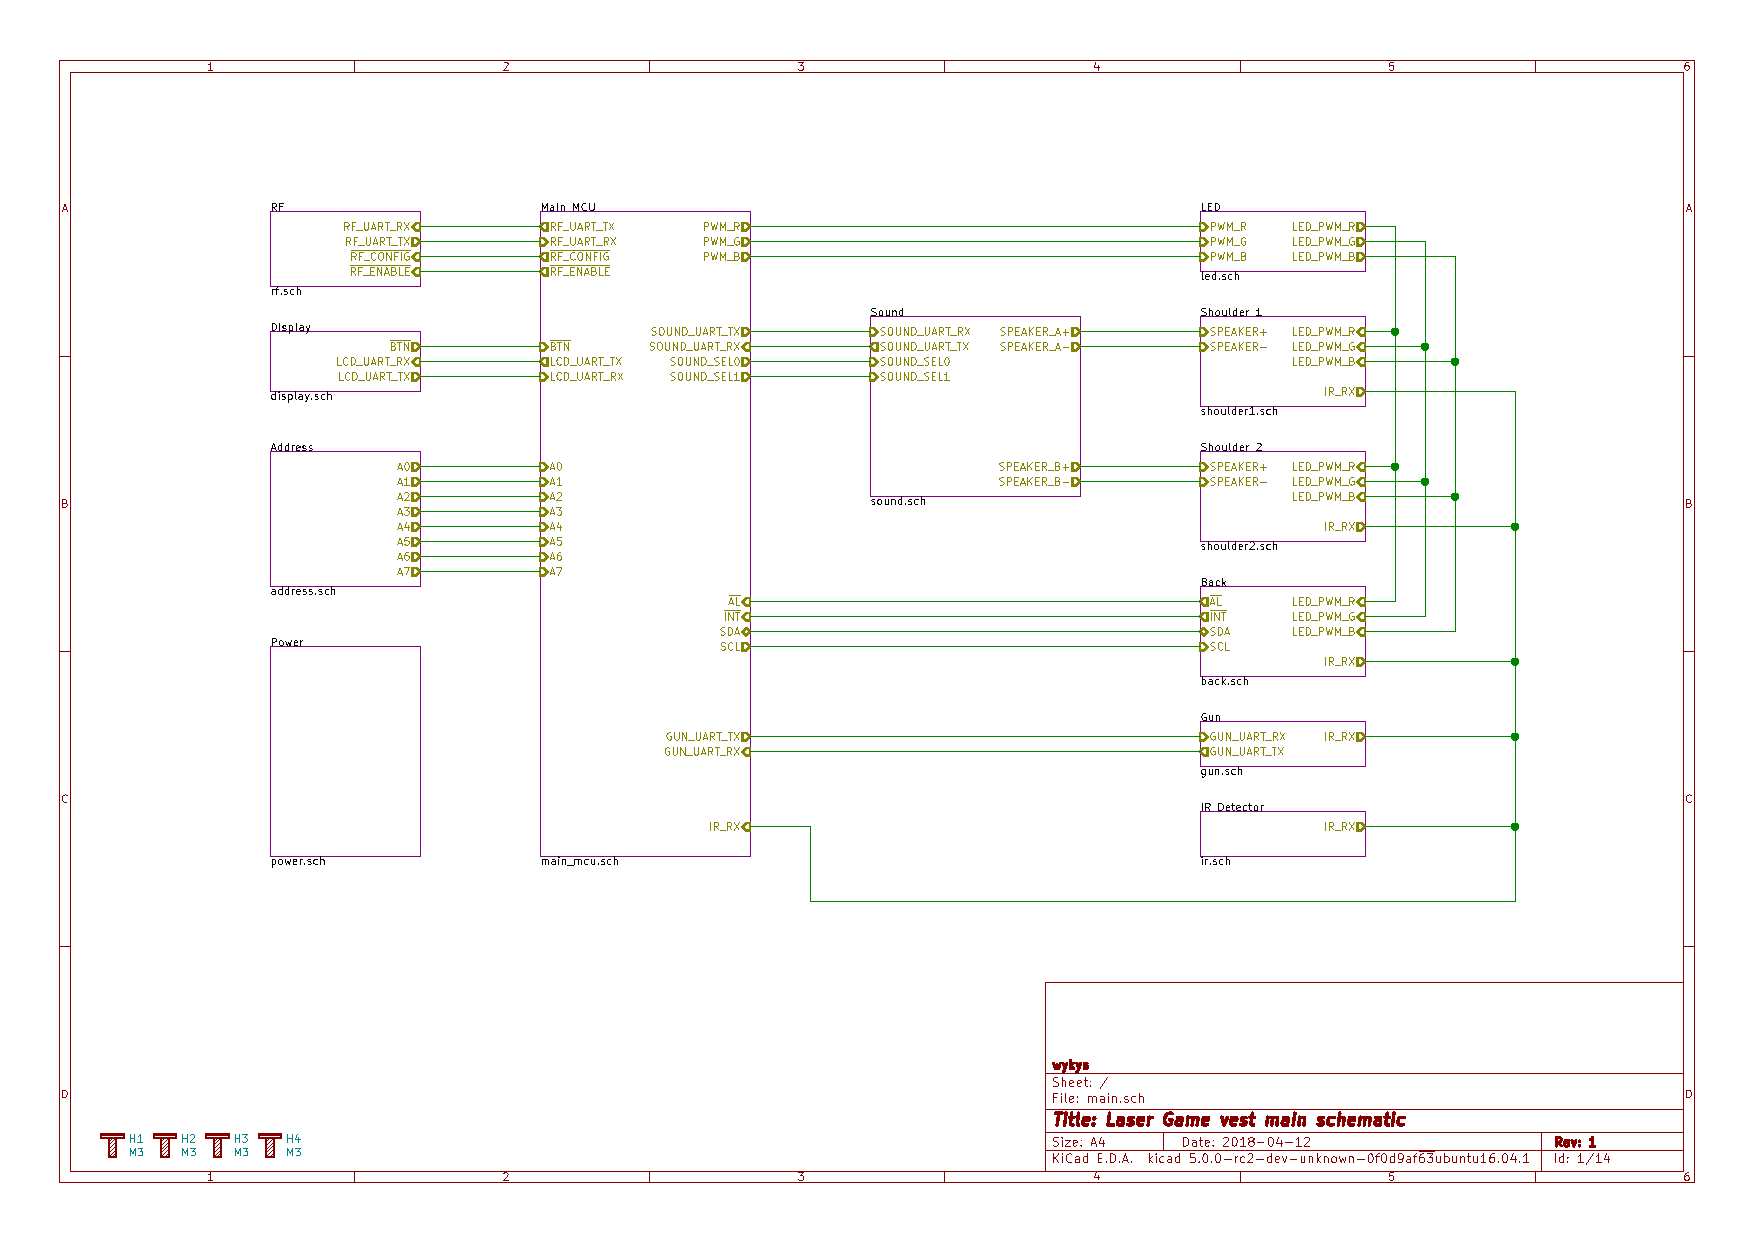
\includegraphics[page=1, height=\textwidth]{sch/main}
        \caption{Schéma zapojení hlavní desky vesty strana 1}
    \end{figure}
\end{landscape}
\begin{landscape}
    \begin{figure}[h]
        \centering
        \includegraphics[page=2, height=\textwidth]{sch/main}
        \caption{Schéma zapojení hlavní desky vesty strana 2}
    \end{figure}
\end{landscape}
\begin{landscape}
    \begin{figure}[h]
        \centering
        \includegraphics[page=3, height=\textwidth]{sch/main}
        \caption{Schéma zapojení hlavní desky vesty strana 3}
    \end{figure}
\end{landscape}
\begin{landscape}
    \begin{figure}[h]
        \centering
        \includegraphics[page=4, height=\textwidth]{sch/main}
        \caption{Schéma zapojení hlavní desky vesty strana 4}
    \end{figure}
\end{landscape}
\begin{landscape}
    \begin{figure}[h]
        \centering
        \includegraphics[page=5, height=\textwidth]{sch/main}
        \caption{Schéma zapojení hlavní desky vesty strana 5}
    \end{figure}
\end{landscape}
\begin{landscape}
    \begin{figure}[h]
        \centering
        \includegraphics[page=6, height=\textwidth]{sch/main}
        \caption{Schéma zapojení hlavní desky vesty strana 6}
    \end{figure}
\end{landscape}
\begin{landscape}
    \begin{figure}[h]
        \centering
        \includegraphics[page=7, height=\textwidth]{sch/main}
        \caption{Schéma zapojení hlavní desky vesty strana 7}
    \end{figure}
\end{landscape}
\begin{landscape}
    \begin{figure}[h]
        \centering
        \includegraphics[page=8, height=\textwidth]{sch/main}
        \caption{Schéma zapojení hlavní desky vesty strana 8}
    \end{figure}
\end{landscape}
\begin{landscape}
    \begin{figure}[h]
        \centering
        \includegraphics[page=9, height=\textwidth]{sch/main}
        \caption{Schéma zapojení hlavní desky vesty strana 9}
    \end{figure}
\end{landscape}
\begin{landscape}
    \begin{figure}[h]
        \centering
        \includegraphics[page=10, height=\textwidth]{sch/main}
        \caption{Schéma zapojení hlavní desky vesty strana 10}
    \end{figure}
\end{landscape}
\begin{landscape}
    \begin{figure}[h]
        \centering
        \includegraphics[page=11, height=\textwidth]{sch/main}
        \caption{Schéma zapojení hlavní desky vesty strana 11}
    \end{figure}
\end{landscape}
\begin{landscape}
    \begin{figure}[h]
        \centering
        \includegraphics[page=12, height=\textwidth]{sch/main}
        \caption{Schéma zapojení hlavní desky vesty strana 12}
    \end{figure}
\end{landscape}
\begin{landscape}
    \begin{figure}[h]
        \centering
        \includegraphics[page=13, height=\textwidth]{sch/main}
        \caption{Schéma zapojení hlavní desky vesty strana 13}
    \end{figure}
\end{landscape}
\begin{landscape}
    \begin{figure}[h]
        \centering
        \includegraphics[page=14, height=\textwidth]{sch/main}
        \caption{Schéma zapojení hlavní desky vesty strana 14}
    \end{figure}
\end{landscape}


\begin{landscape}
    \begin{figure}[h]
        \centering
        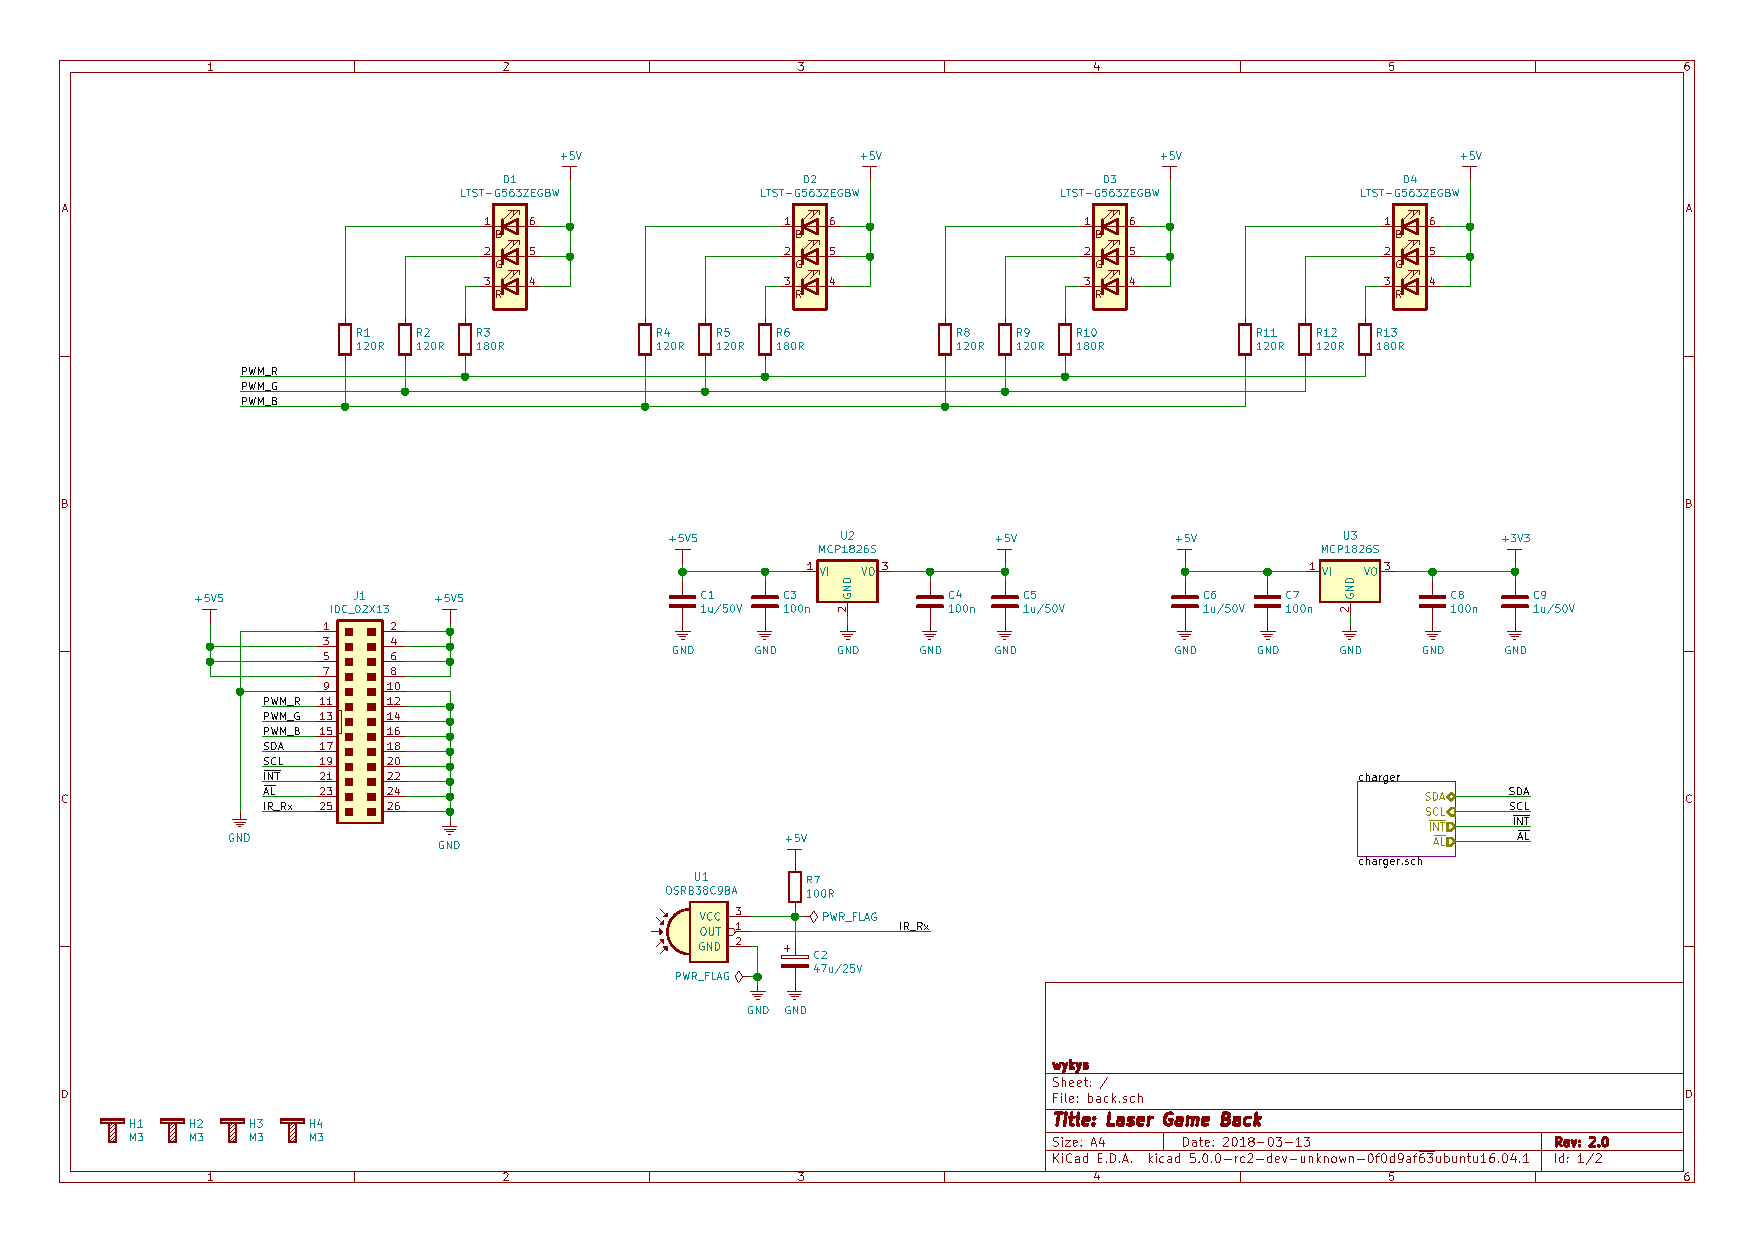
\includegraphics[page=1, height=\textwidth]{sch/back}
        \caption{Schéma zapojení nabíječky vesty strana 1}
    \end{figure}
\end{landscape}
\begin{landscape}
    \begin{figure}[h]
        \centering
        \includegraphics[page=2, height=\textwidth]{sch/back}
        \caption{Schéma zapojení nabíječky vesty strana 2}
    \end{figure}
\end{landscape}


\begin{landscape}
    \begin{figure}[h]
        \centering
        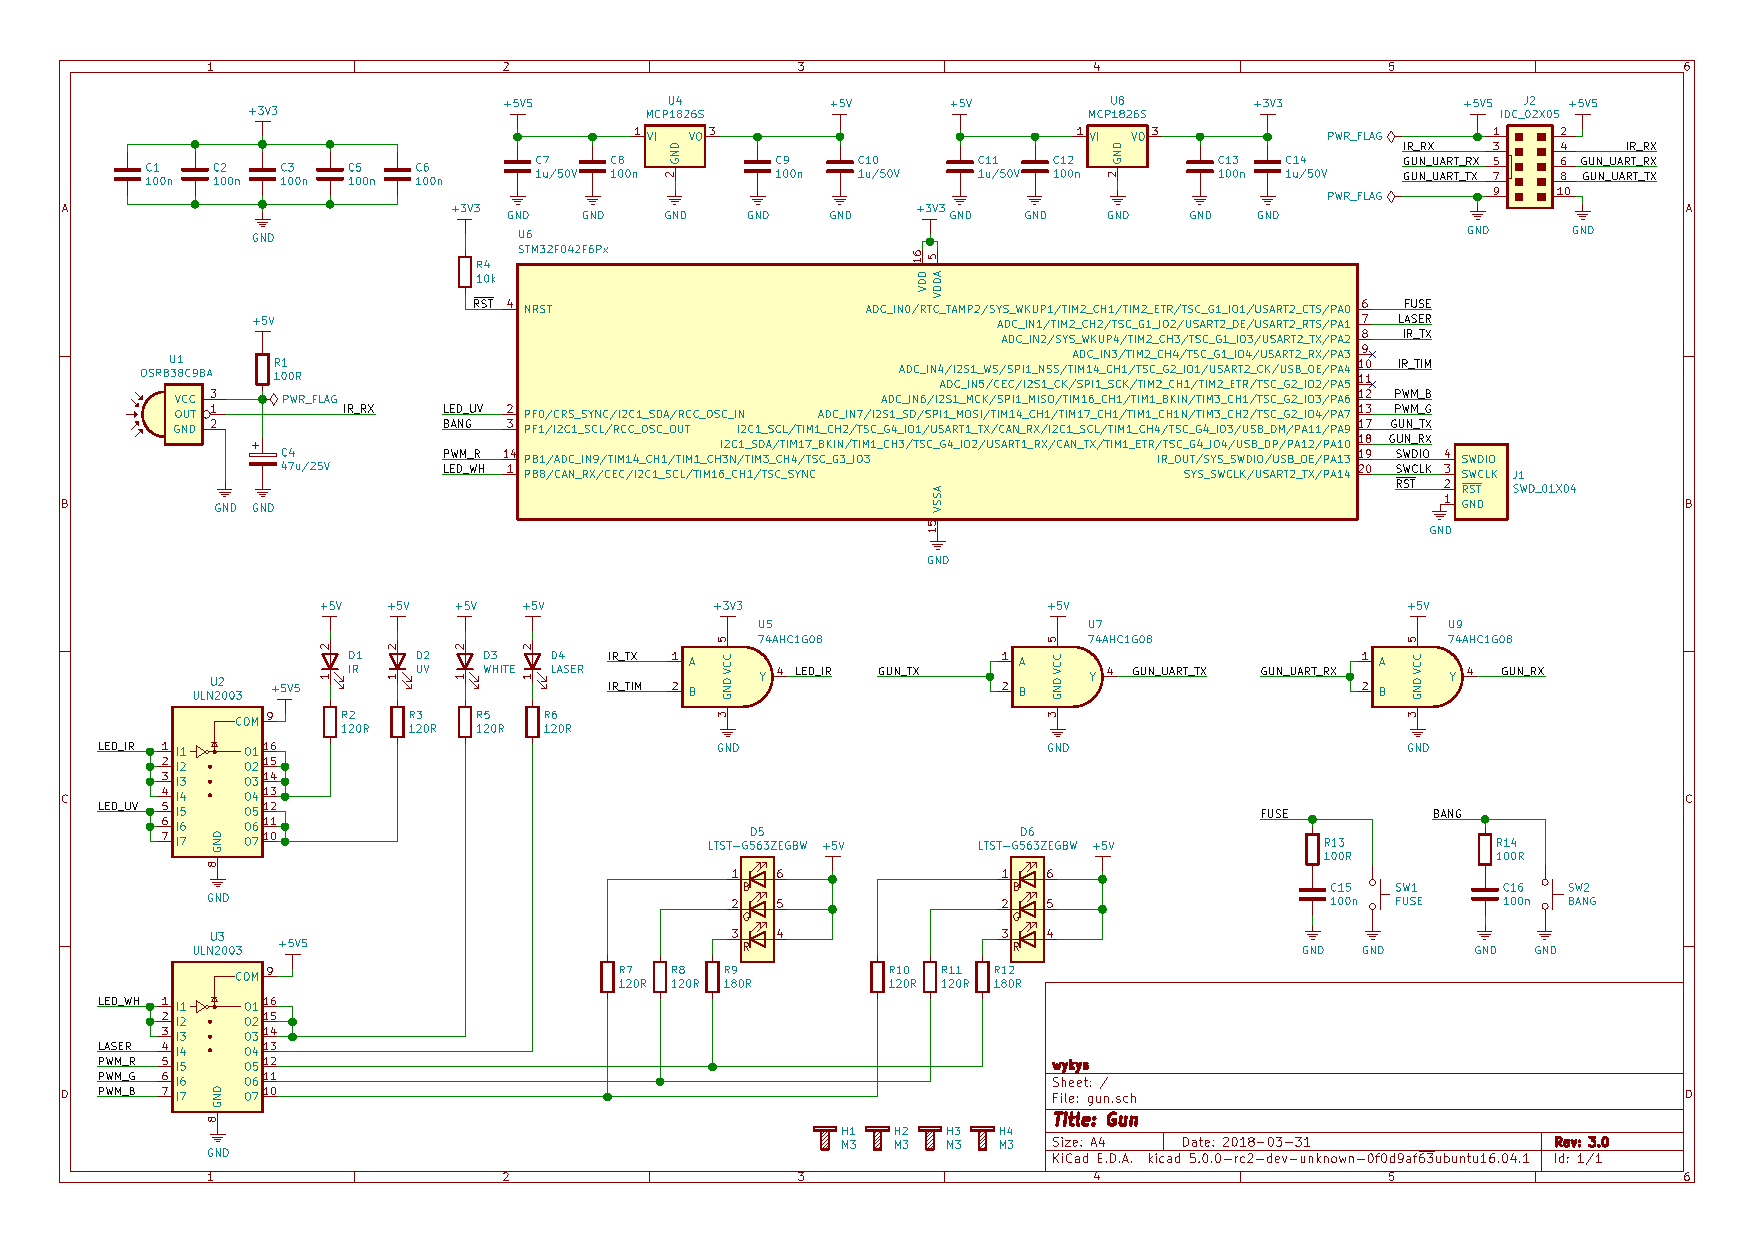
\includegraphics[page=1, height=\textwidth]{sch/gun}
        \caption{Schéma zapojení zbraně}
    \end{figure}
\end{landscape}


\begin{landscape}
    \begin{figure}[h]
        \centering
        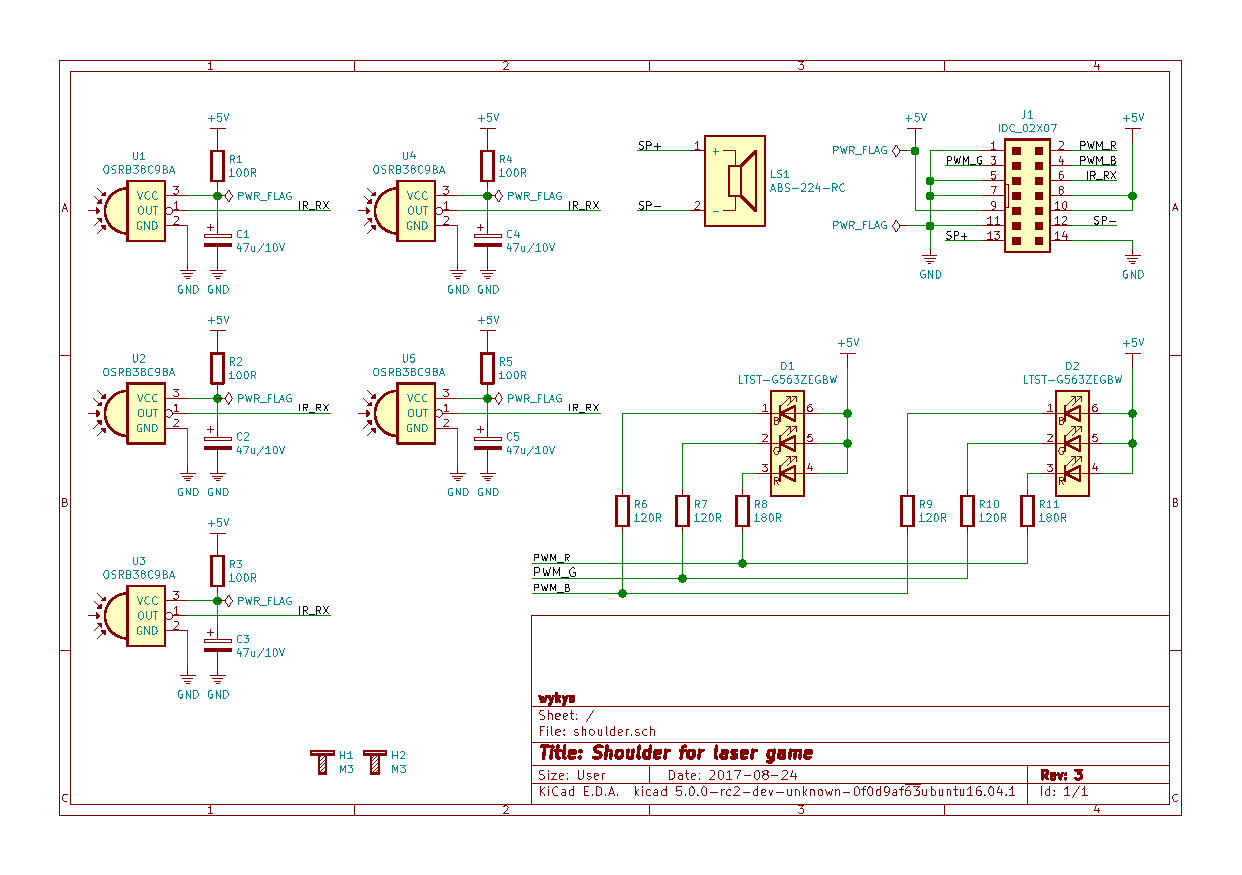
\includegraphics[page=1, height=\textwidth]{sch/shoulder}
        \caption{Schéma zapojení desky na rameno}
    \end{figure}
\end{landscape}


\begin{landscape}
    \begin{figure}[h]
        \centering
        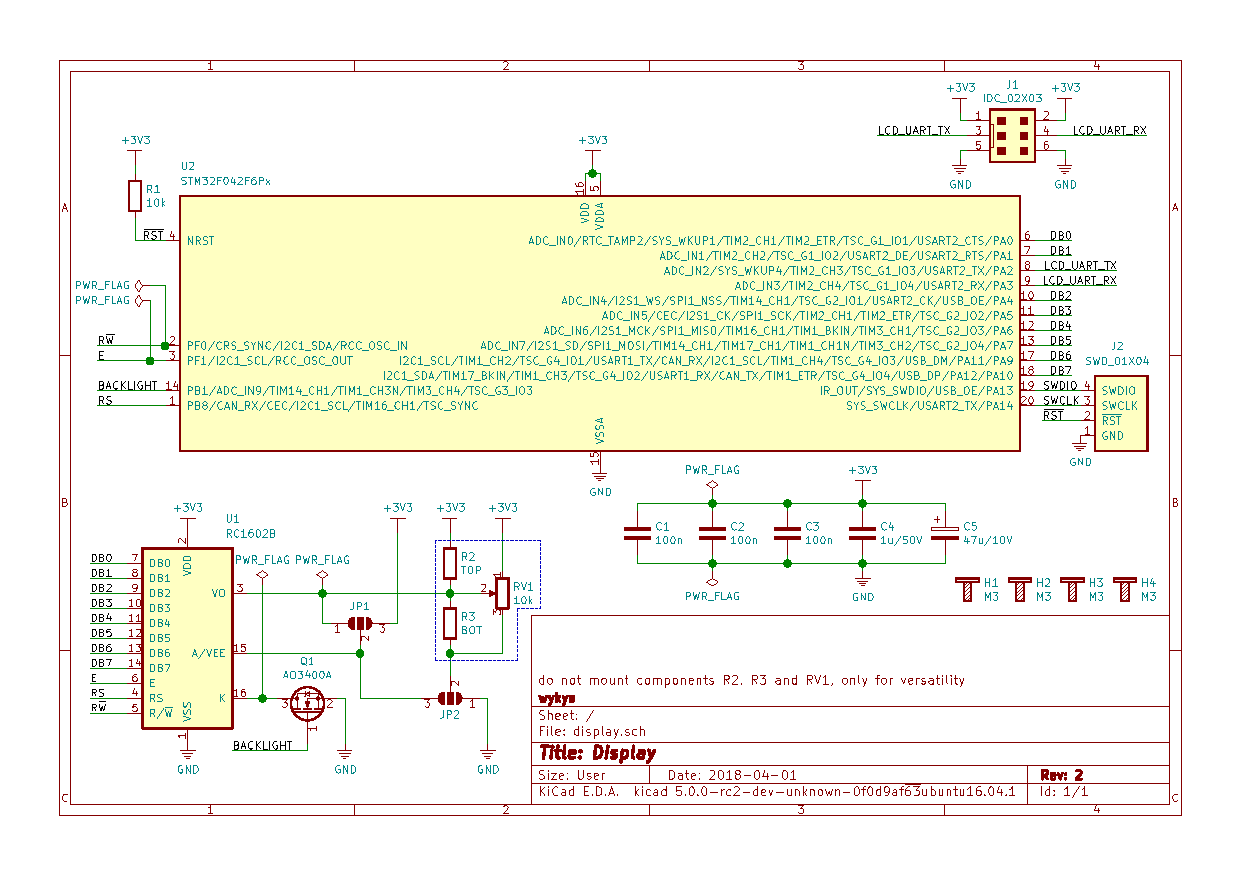
\includegraphics[page=1, height=\textwidth]{sch/display}
        \caption{Schéma zapojení zobrazovače}
    \end{figure}
\end{landscape}


\begin{landscape}
    \begin{figure}[h]
        \centering
        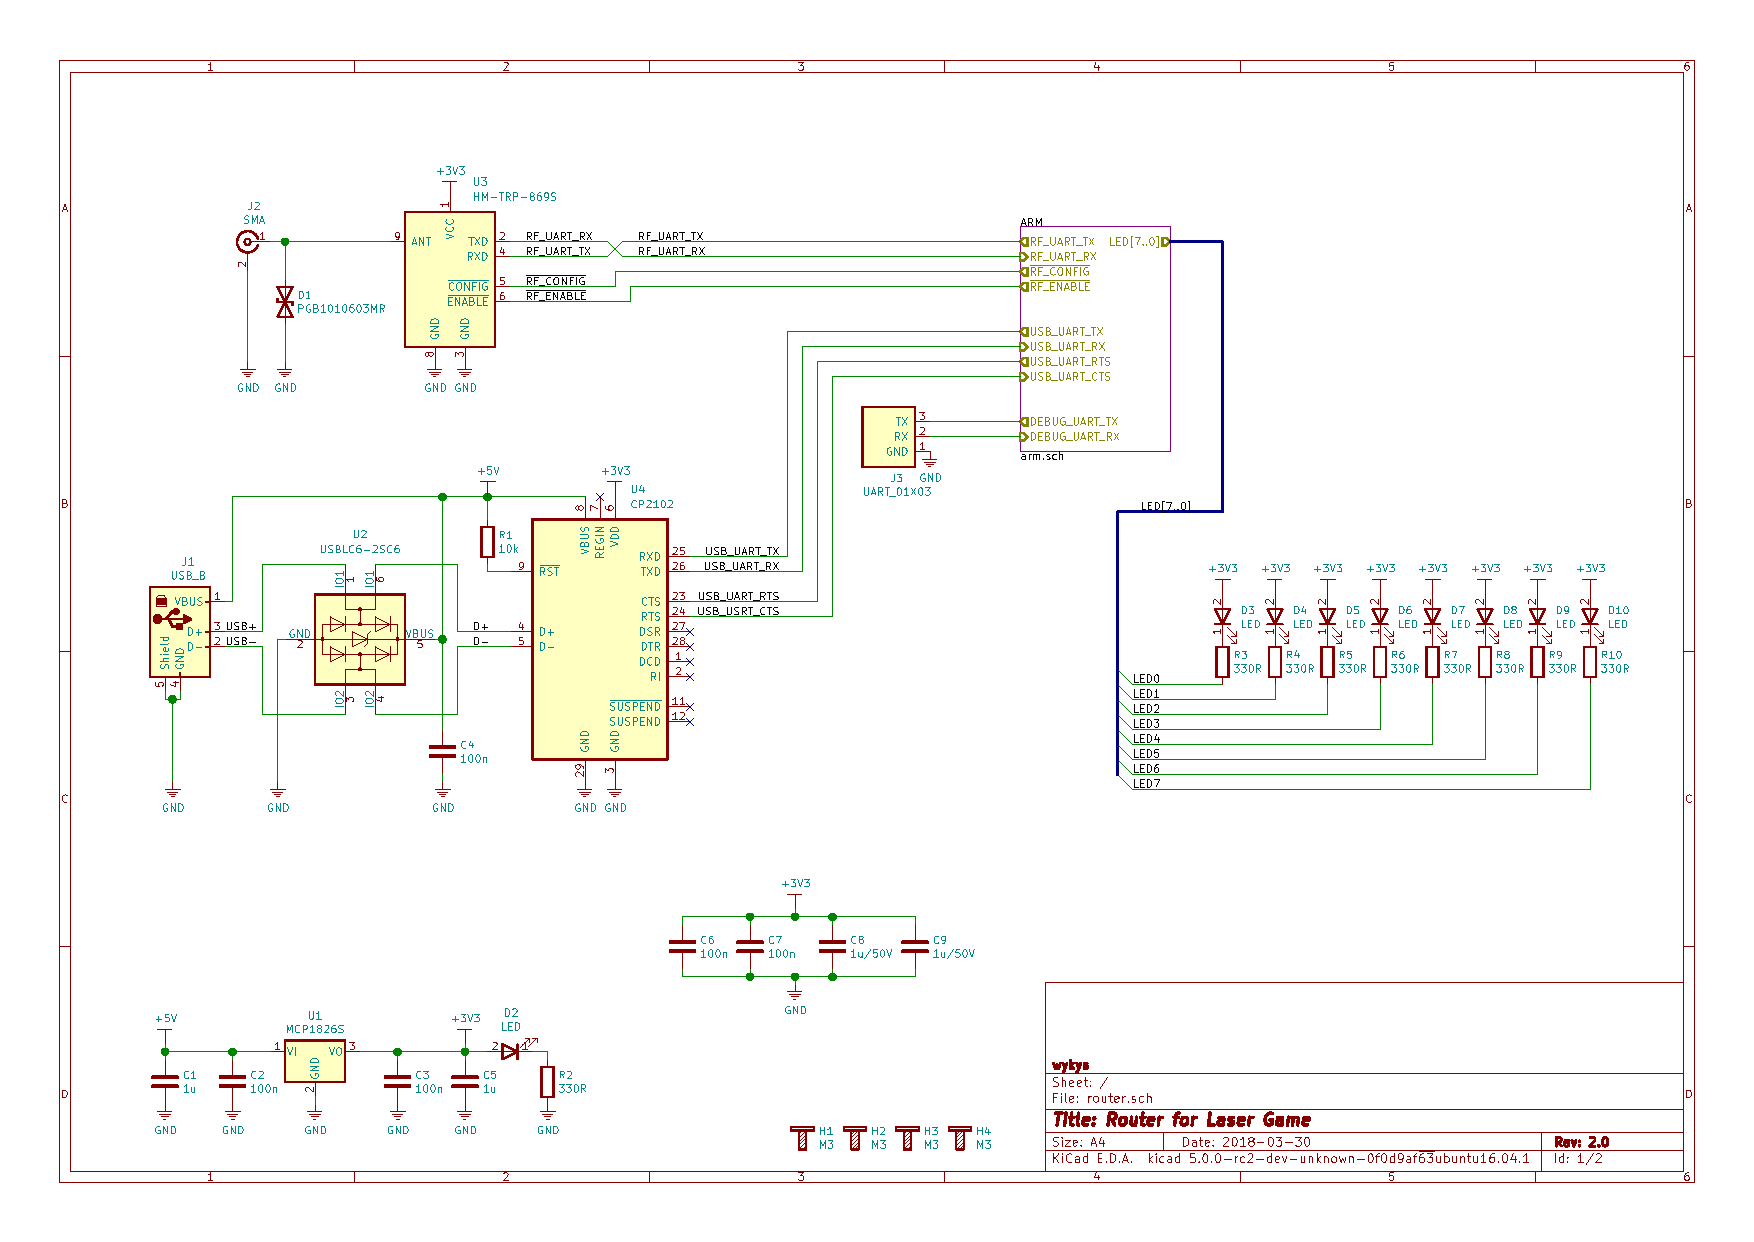
\includegraphics[page=1, height=\textwidth]{sch/router}
        \caption{Schéma zapojení směrovače strana 1}
    \end{figure}
\end{landscape}
\begin{landscape}
    \begin{figure}[h]
        \centering
        \includegraphics[page=2, height=\textwidth]{sch/router}
        \caption{Schéma zapojení směrovače strana 2}
    \end{figure}
\end{landscape}


\chapter{Přiložené osazovací plány}
\begin{figure}[h]
    \centering
    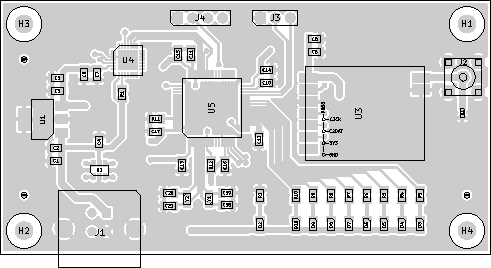
\includegraphics[page=1, width=0.99\textwidth]{pcb/router-placement}
    \caption{Osazovací plán směrovače}
\end{figure}
\begin{figure}[h]
    \centering
    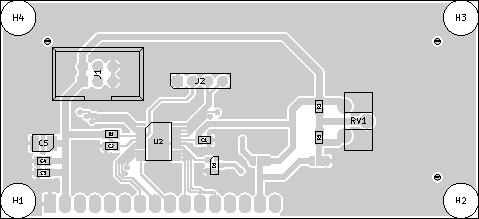
\includegraphics[page=1, width=0.99\textwidth]{pcb/display-placement}
    \caption{Osazovací plán zobrazovací jednotky}
\end{figure}
\begin{figure}[h]
    \centering
    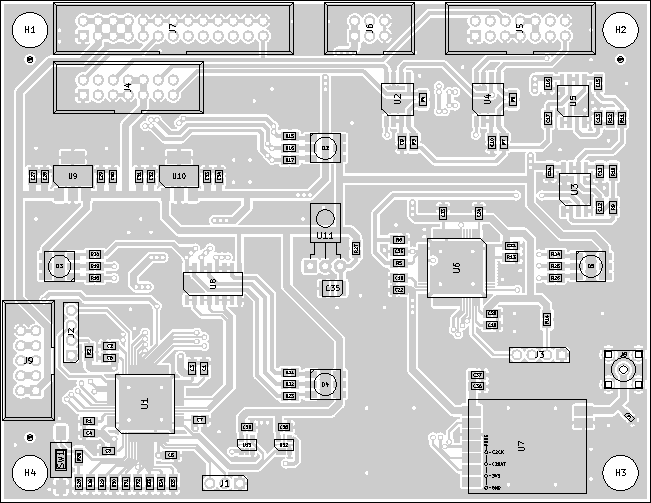
\includegraphics[page=1, width=\textwidth]{pcb/main-placement}
    \caption{Osazovací plán hlavní desky}
\end{figure}
\begin{figure}[h]
    \centering
    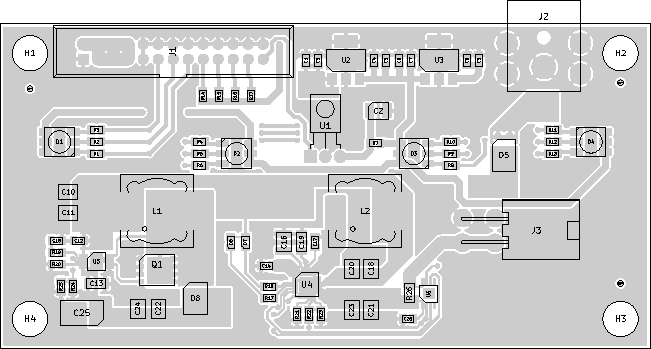
\includegraphics[page=1, width=\textwidth]{pcb/back-placement}
    \caption{Osazovací plán desky na záda}
\end{figure}
\begin{figure}[h]
    \centering
    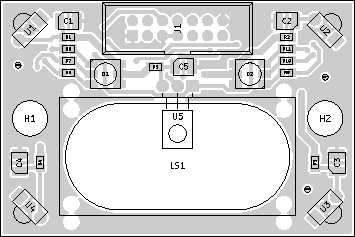
\includegraphics[page=1, width=\textwidth]{pcb/shoulder-placement}
    \caption{Osazovací plán desky na rameno}
\end{figure}
\begin{figure}[h]
    \centering
    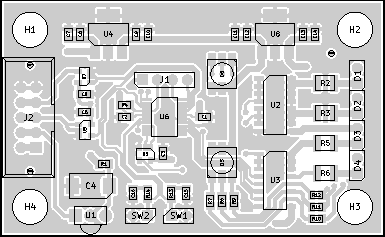
\includegraphics[page=1, width=\textwidth]{pcb/gun-placement}
    \caption{Osazovací plán zbraně}
\end{figure}


\chapter{Přiložené výkresy plošných spojů}
\begin{figure}[h]
    \centering
    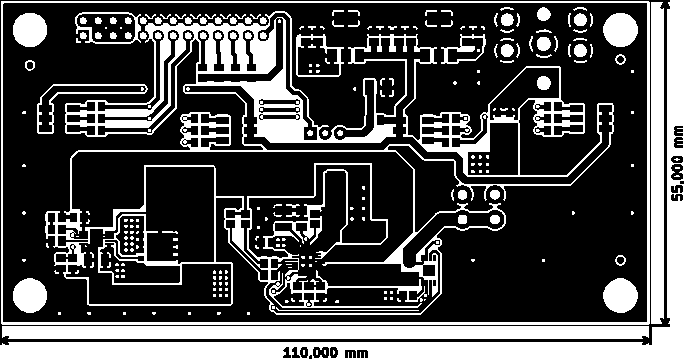
\includegraphics{pcb/back-top}
    \caption{Plošný spoj desky na záda v měřítku 1:1, pohled ze strany součástek}
\end{figure}
\begin{figure}[h]
    \centering
    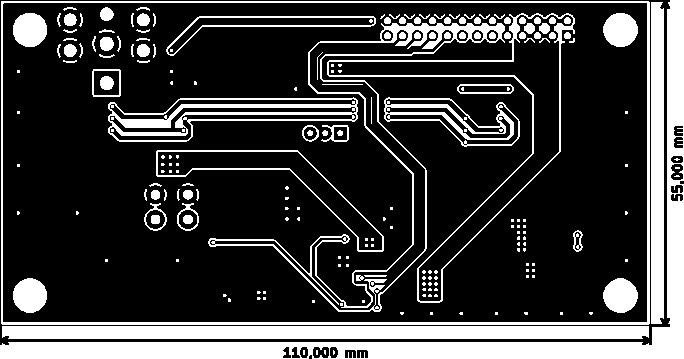
\includegraphics{pcb/back-bot}
    \caption{Plošný spoj desky na záda v měřítku 1:1, pohled ze strany spojů}
\end{figure}

\begin{figure}[h]
    \centering
    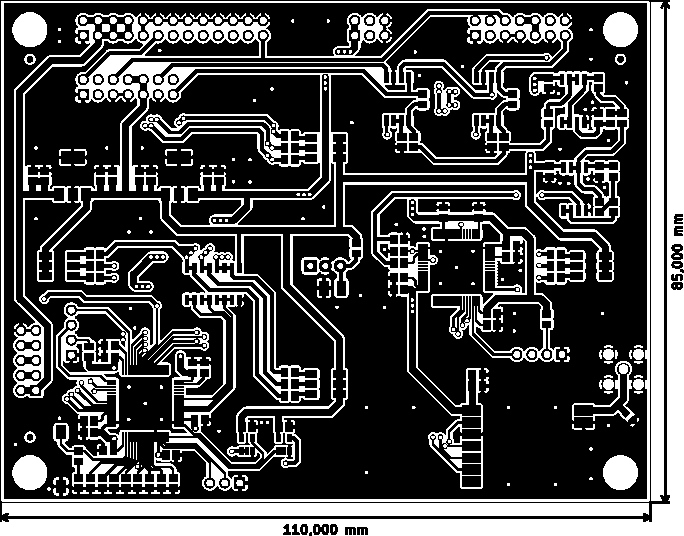
\includegraphics{pcb/main-top}
    \caption{Plošný spoj hlavní desky v měřítku 1:1, pohled ze strany součástek}
\end{figure}
\begin{figure}[h]
    \centering
    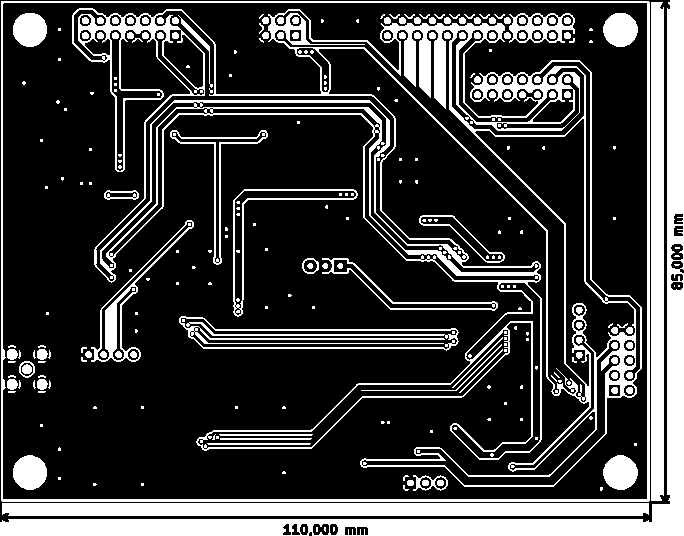
\includegraphics{pcb/main-bot}
    \caption{Plošný spoj hlavní desky v měřítku 1:1, pohled ze strany spojů}
\end{figure}

\begin{figure}[h]
    \centering
    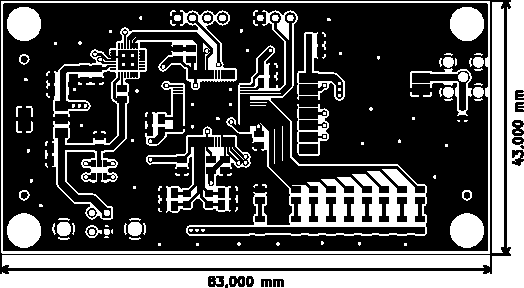
\includegraphics{pcb/router-top}
    \caption{Plošný spoj směrovače v měřítku 1:1, pohled ze strany součástek}
\end{figure}
\begin{figure}[h]
    \centering
    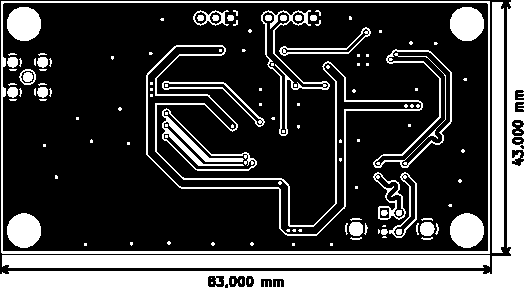
\includegraphics{pcb/router-bot}
    \caption{Plošný spoj směrovače v měřítku 1:1, pohled ze strany spojů}
\end{figure}

\begin{figure}[h]
    \centering
    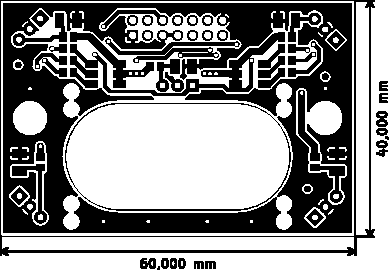
\includegraphics{pcb/shoulder-top}
    \caption{Plošný spoj desky na rameno v měřítku 1:1, pohled ze strany součástek}
\end{figure}
\begin{figure}[h]
    \centering
    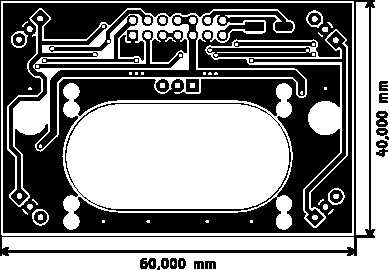
\includegraphics{pcb/shoulder-bot}
    \caption{Plošný spoj desky na rameno v měřítku 1:1, pohled ze strany spojů}
\end{figure}

\begin{figure}[h]
    \centering
    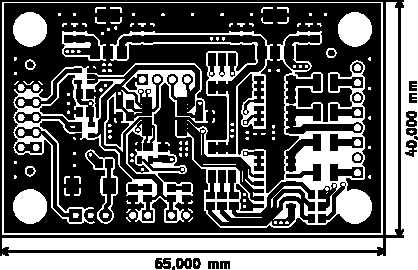
\includegraphics{pcb/gun-top}
    \caption{Plošný spoj zbraně v měřítku 1:1, pohled ze strany součástek}
\end{figure}
\begin{figure}[h]
    \centering
    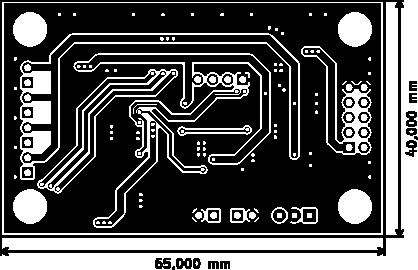
\includegraphics{pcb/gun-bot}
    \caption{Plošný spoj zbraně v měřítku 1:1, pohled ze strany spojů}
\end{figure}

\begin{figure}[h]
    \centering
    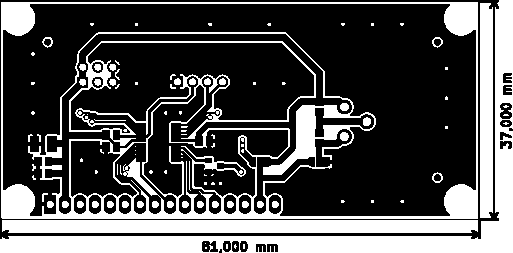
\includegraphics{pcb/display-top}
    \caption{Plošný spoj zobrazovací jednotky v měřítku 1:1, pohled ze strany součástek}
\end{figure}
\begin{figure}[h]
    \centering
    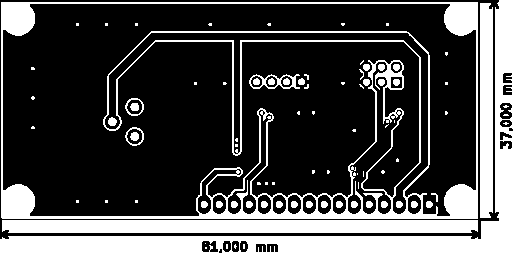
\includegraphics{pcb/display-bot}
    \caption{Plošný spoj zobrazovací jednotky v měřítku 1:1, pohled ze strany spojů}
\end{figure}


\chapter{Foto dokumentace}
\begin{figure}[h]
    \centering
    \includegraphics[width=0.84\textwidth]{foto/set-rotation}
    \caption{Kompletní sada elektroniky pro jednoho hráče}
\end{figure}


% Konec dokumentu
\end{document}
